\section{Results}\label{sec:results}

\begin{table}[tbp]
\centering
\scriptsize
\caption{Honest runs ($K=5$): test AUC and soft DPD (lower is fairer), mean$\pm$sd over 10 seeds. Baselines and CLAMP (sums channel) are the runs of the earlier study, with the output-rule warm-up applied; CLAMP used $P=1$ on Bail, Credit, Pokec-z, Pokec-n and AMiner-S and $P=10$ on German, NBA and Facebook, whereas CLAMP-RT uses $P=10$ everywhere. $^{c}$: reads per-client fairness quantities or group rates in the clear. PUFFLE and FedFDP barely learn at their privacy level (AUC near 0.5).}
\label{tab:e1}
\resizebox{\textwidth}{!}{%
\begin{tabular}{lcccccccc}
\toprule
 & \multicolumn{2}{c}{German} & \multicolumn{2}{c}{Bail} & \multicolumn{2}{c}{Credit} & \multicolumn{2}{c}{Pokec-z} \\
 & AUC & DPD & AUC & DPD & AUC & DPD & AUC & DPD \\
\midrule
FedAvg-GAT & 0.76$\pm$0.05 & 0.110$\pm$0.058 & 0.80$\pm$0.04 & 0.019$\pm$0.011 & 0.77$\pm$0.01 & 0.078$\pm$0.010 & 0.74$\pm$0.02 & 0.031$\pm$0.013 \\
FairFed$^{c}$ & 0.75$\pm$0.05 & 0.049$\pm$0.039 & 0.80$\pm$0.03 & 0.012$\pm$0.007 & 0.75$\pm$0.01 & 0.008$\pm$0.005 & 0.64$\pm$0.05 & 0.004$\pm$0.003 \\
F$^2$GNN$^{c}$ & 0.73$\pm$0.02 & 0.042$\pm$0.030 & 0.78$\pm$0.03 & 0.012$\pm$0.008 & 0.76$\pm$0.01 & 0.006$\pm$0.007 & 0.74$\pm$0.02 & 0.008$\pm$0.007 \\
FairGFL & 0.74$\pm$0.05 & 0.081$\pm$0.070 & 0.78$\pm$0.03 & 0.015$\pm$0.006 & 0.76$\pm$0.01 & 0.072$\pm$0.009 & 0.66$\pm$0.02 & 0.041$\pm$0.011 \\
FedGraph-Fair & 0.66$\pm$0.09 & 0.080$\pm$0.051 & 0.76$\pm$0.03 & 0.010$\pm$0.007 & 0.75$\pm$0.01 & 0.075$\pm$0.014 & 0.64$\pm$0.03 & 0.039$\pm$0.013 \\
FedFACT$^{c}$ & 0.72$\pm$0.04 & 0.078$\pm$0.064 & 0.80$\pm$0.03 & 0.013$\pm$0.008 & 0.75$\pm$0.01 & 0.070$\pm$0.016 & 0.63$\pm$0.04 & 0.024$\pm$0.014 \\
PUFFLE & 0.49$\pm$0.08 & 0.011$\pm$0.007 & 0.50$\pm$0.06 & 0.003$\pm$0.003 & 0.46$\pm$0.13 & 0.016$\pm$0.008 & 0.55$\pm$0.11 & 0.008$\pm$0.009 \\
FedFDP & 0.53$\pm$0.09 & 0.014$\pm$0.021 & 0.51$\pm$0.03 & 0.004$\pm$0.003 & 0.54$\pm$0.11 & 0.017$\pm$0.009 & 0.64$\pm$0.11 & 0.008$\pm$0.008 \\
FairGNN & 0.57$\pm$0.06 & 0.111$\pm$0.082 & 0.56$\pm$0.09 & 0.019$\pm$0.020 & 0.67$\pm$0.09 & 0.100$\pm$0.055 & 0.54$\pm$0.08 & 0.005$\pm$0.013 \\
FairSIN & 0.72$\pm$0.05 & 0.092$\pm$0.062 & 0.79$\pm$0.03 & 0.025$\pm$0.008 & 0.75$\pm$0.00 & 0.070$\pm$0.012 & 0.66$\pm$0.05 & 0.026$\pm$0.010 \\
ClipMean (no controller) & 0.73$\pm$0.06 & 0.088$\pm$0.069 & 0.78$\pm$0.03 & 0.016$\pm$0.009 & 0.77$\pm$0.01 & 0.071$\pm$0.009 & 0.75$\pm$0.02 & 0.042$\pm$0.011 \\
\midrule
CLAMP (sums channel) & 0.72$\pm$0.06 & 0.058$\pm$0.044 & 0.78$\pm$0.03 & 0.016$\pm$0.009 & 0.76$\pm$0.01 & 0.018$\pm$0.015 & 0.75$\pm$0.02 & 0.026$\pm$0.004 \\
CLAMP-GCN (sums channel) & 0.73$\pm$0.05 & 0.065$\pm$0.044 & 0.79$\pm$0.02 & 0.015$\pm$0.006 & 0.75$\pm$0.01 & 0.014$\pm$0.013 & 0.72$\pm$0.02 & 0.028$\pm$0.006 \\
\midrule
CLAMP-RT, no bias correction & 0.51$\pm$0.06 & 0.602$\pm$0.084 & 0.77$\pm$0.04 & 0.014$\pm$0.008 & 0.76$\pm$0.01 & 0.049$\pm$0.041 & 0.76$\pm$0.03 & 0.032$\pm$0.011 \\
CLAMP-RT-GCN & 0.71$\pm$0.07 & 0.172$\pm$0.198 & 0.79$\pm$0.03 & 0.014$\pm$0.007 & 0.76$\pm$0.01 & 0.059$\pm$0.017 & 0.74$\pm$0.02 & 0.041$\pm$0.009 \\
\textbf{CLAMP-RT} & 0.72$\pm$0.07 & 0.172$\pm$0.189 & 0.78$\pm$0.03 & 0.015$\pm$0.010 & 0.77$\pm$0.01 & 0.061$\pm$0.017 & 0.76$\pm$0.03 & 0.037$\pm$0.011 \\
\bottomrule
\end{tabular}}
\vspace{4pt}
\resizebox{\textwidth}{!}{%
\begin{tabular}{lcccccccc}
\toprule
 & \multicolumn{2}{c}{Pokec-n} & \multicolumn{2}{c}{AMiner-S} & \multicolumn{2}{c}{NBA} & \multicolumn{2}{c}{Facebook} \\
 & AUC & DPD & AUC & DPD & AUC & DPD & AUC & DPD \\
\midrule
FedAvg-GAT & 0.75$\pm$0.02 & 0.034$\pm$0.017 & 0.94$\pm$0.00 & 0.007$\pm$0.004 & 0.81$\pm$0.06 & 0.099$\pm$0.059 & 0.77$\pm$0.05 & 0.078$\pm$0.048 \\
FairFed$^{c}$ & 0.62$\pm$0.06 & 0.006$\pm$0.004 & 0.94$\pm$0.00 & 0.005$\pm$0.003 & 0.80$\pm$0.05 & 0.081$\pm$0.062 & 0.76$\pm$0.03 & 0.049$\pm$0.031 \\
F$^2$GNN$^{c}$ & 0.74$\pm$0.03 & 0.008$\pm$0.007 & 0.94$\pm$0.01 & 0.005$\pm$0.004 & 0.78$\pm$0.13 & 0.109$\pm$0.072 & 0.76$\pm$0.05 & 0.069$\pm$0.040 \\
FairGFL & 0.65$\pm$0.03 & 0.044$\pm$0.007 & 0.94$\pm$0.01 & 0.003$\pm$0.002 & 0.76$\pm$0.04 & 0.078$\pm$0.044 & 0.75$\pm$0.05 & 0.080$\pm$0.040 \\
FedGraph-Fair & 0.59$\pm$0.05 & 0.024$\pm$0.015 & 0.93$\pm$0.01 & 0.003$\pm$0.003 & 0.77$\pm$0.10 & 0.084$\pm$0.043 & 0.74$\pm$0.05 & 0.094$\pm$0.037 \\
FedFACT$^{c}$ & 0.59$\pm$0.06 & 0.012$\pm$0.011 & 0.92$\pm$0.01 & 0.008$\pm$0.004 & 0.76$\pm$0.04 & 0.142$\pm$0.082 & 0.74$\pm$0.05 & 0.055$\pm$0.042 \\
PUFFLE & 0.57$\pm$0.11 & 0.010$\pm$0.006 & 0.49$\pm$0.03 & 0.006$\pm$0.005 & 0.37$\pm$0.19 & 0.014$\pm$0.012 & 0.53$\pm$0.10 & 0.009$\pm$0.006 \\
FedFDP & 0.66$\pm$0.08 & 0.010$\pm$0.008 & 0.49$\pm$0.03 & 0.006$\pm$0.004 & 0.39$\pm$0.20 & 0.015$\pm$0.010 & 0.54$\pm$0.08 & 0.013$\pm$0.009 \\
FairGNN & 0.50$\pm$0.00 & 0.000$\pm$0.000 & 0.63$\pm$0.08 & 0.098$\pm$0.035 & 0.77$\pm$0.08 & 0.097$\pm$0.044 & 0.51$\pm$0.05 & 0.024$\pm$0.041 \\
FairSIN & 0.64$\pm$0.06 & 0.043$\pm$0.014 & 0.92$\pm$0.01 & 0.005$\pm$0.003 & 0.73$\pm$0.08 & 0.087$\pm$0.059 & 0.74$\pm$0.05 & 0.070$\pm$0.033 \\
ClipMean (no controller) & 0.75$\pm$0.02 & 0.052$\pm$0.016 & 0.94$\pm$0.01 & 0.005$\pm$0.004 & 0.78$\pm$0.08 & 0.093$\pm$0.068 & 0.77$\pm$0.06 & 0.086$\pm$0.043 \\
\midrule
CLAMP (sums channel) & 0.76$\pm$0.02 & 0.028$\pm$0.012 & 0.94$\pm$0.01 & 0.004$\pm$0.004 & 0.80$\pm$0.08 & 0.076$\pm$0.054 & 0.76$\pm$0.06 & 0.069$\pm$0.034 \\
CLAMP-GCN (sums channel) & 0.71$\pm$0.02 & 0.027$\pm$0.008 & 0.94$\pm$0.00 & 0.002$\pm$0.002 & 0.78$\pm$0.07 & 0.077$\pm$0.044 & 0.76$\pm$0.04 & 0.078$\pm$0.030 \\
\midrule
CLAMP-RT, no bias correction & 0.77$\pm$0.02 & 0.041$\pm$0.014 & 0.94$\pm$0.01 & 0.007$\pm$0.005 & 0.68$\pm$0.10 & 0.203$\pm$0.101 & 0.65$\pm$0.08 & 0.114$\pm$0.063 \\
CLAMP-RT-GCN & 0.72$\pm$0.03 & 0.046$\pm$0.012 & 0.94$\pm$0.01 & 0.002$\pm$0.002 & 0.76$\pm$0.08 & 0.116$\pm$0.065 & 0.75$\pm$0.06 & 0.073$\pm$0.025 \\
\textbf{CLAMP-RT} & 0.76$\pm$0.02 & 0.047$\pm$0.015 & 0.94$\pm$0.01 & 0.004$\pm$0.004 & 0.79$\pm$0.08 & 0.067$\pm$0.050 & 0.76$\pm$0.06 & 0.080$\pm$0.054 \\
\bottomrule
\end{tabular}}
\end{table}

\begin{table}[tbp]
\centering
\scriptsize
\setlength{\tabcolsep}{3pt}
\caption{Statistics channel of CLAMP-RT in the honest runs ($K=5$, $b=1$, $\varepsilon=8$, $R=10$ releases, 10 seeds). $n_{0,\min}$ and $\sigma_d$: range over seeds. Radius: $\sqrt{\tau^2+2\sigma_d^2}+r_R$ of Theorem~\ref{thm:output} at the median $\sigma_d$ and $\beta=0.05$ (vacuous when $\ge1$). $\Dhat>0$: share of releases with a non-zero bias-corrected magnitude. $\lambda^T$: mean final multiplier. Right block: mean test DPD and AUC of CLAMP (sums channel) and CLAMP-RT, with the two-sided Wilcoxon signed-rank $p$-value paired by seed (unadjusted).}
\label{tab:channel}
\begin{adjustbox}{max width=\textwidth}
\begin{tabular}{lccccc|ccc|ccc}
\toprule
Dataset & $n_{0,\min}$ & $\sigma_d$ & Radius & $\Dhat>0$ & $\lambda^T$ & \multicolumn{3}{c|}{DPD: CLAMP / RT / $p$} & \multicolumn{3}{c}{AUC: CLAMP / RT / $p$} \\
\midrule
German & 1--2 & 0.672--1.345 & 8.48 & 0.31 & 2.27 & 0.058 & 0.172 & 0.064 & 0.721 & 0.719 & 0.695 \\
Bail & 13--26 & 0.052--0.103 & 0.59 & 0.29 & 0.09 & 0.016 & 0.015 & 0.193 & 0.778 & 0.776 & 0.922 \\
Credit & 19--29 & 0.046--0.071 & 0.40 & 0.42 & 0.08 & 0.018 & 0.061 & 0.002 & 0.760 & 0.769 & 0.002 \\
Pokec-z & 42--105 & 0.013--0.032 & 0.19 & 0.45 & 0.03 & 0.026 & 0.037 & 0.014 & 0.753 & 0.757 & 0.049 \\
Pokec-n & 41--64 & 0.021--0.033 & 0.19 & 0.59 & 0.06 & 0.028 & 0.047 & 0.002 & 0.758 & 0.764 & 0.275 \\
AMiner-S & 25--44 & 0.031--0.054 & 0.29 & 0.28 & 0.02 & 0.004 & 0.004 & 0.557 & 0.942 & 0.941 & 0.037 \\
NBA & 1--1 & 1.345--1.345 & 8.48 & 0.29 & 2.86 & 0.076 & 0.067 & 0.492 & 0.796 & 0.788 & 0.391 \\
Facebook & 1--2 & 0.672--1.345 & 8.48 & 0.28 & 2.85 & 0.069 & 0.080 & 0.557 & 0.762 & 0.764 & 0.557 \\
\bottomrule
\end{tabular}
\end{adjustbox}
\end{table}


\subsection{Honest runs}\label{sec:main}

Table~\ref{tab:e1} reports AUC and $\dpd$ of all methods without attack, and Table~\ref{tab:channel} the state of the gap channel and the paired comparison with \clamp{}.

\paragraph{Where the budget binds, \rt{} controls the gap less tightly than \clamp{}}
On Credit, Pokec-z and Pokec-n the unconstrained clipped model has a gap above $\tau=0.03$ (ClipMean 0.071, 0.042 and 0.052). \clamp{} brought it to 0.018, 0.026 and 0.028. \rt{} reaches 0.061, 0.037 and 0.047, significantly higher than \clamp{} on all three graphs ($p=0.002$, $0.014$ and $0.002$), with an AUC that is equal or slightly higher (0.769 against 0.760 on Credit, $p=0.002$; 0.757 against 0.753 on Pokec-z; 0.764 against 0.758 on Pokec-n). Against ClipMean the reduction is small (0.071 to 0.061 on Credit, 0.052 to 0.047 on Pokec-n), and on the two Pokec graphs plain FedAvg-GAT has a lower mean gap (0.031 and 0.034). In the honest setting, \rt{} is therefore a weaker fairness controller than \clamp{}. Two causes are visible in the logs. First, the multiplier stays small: its final value averages 0.03--0.08 on these graphs (Table~\ref{tab:channel}) against 0.17--0.89 for \clamp{} on Credit, because \rt{} updates it ten times instead of a hundred. Second, the noise on one trimmed scalar is large relative to the gap: $\sigma_d$ is 0.046--0.071 on Credit, larger than the budget, and after bias correction 42--59\% of the releases have a non-zero magnitude on these three graphs. The privacy sweep (Section~\ref{sec:privacy}) separates the two causes in part: with per-round releases at $\varepsilon=8$, \rt{} reaches 0.028 and 0.029 on Pokec-z and Pokec-n, the level of \clamp{}, but on Credit per-round releases are worse (0.090). The baselines that read per-client fairness quantities in the clear reach lower gaps than both protocols (F$^2$GNN 0.006--0.008 on these graphs), as in the earlier study.

\paragraph{Where the budget does not bind}
On Bail and AMiner-S the unconstrained gap is already below $\tau$ (0.016 and 0.005), and \rt{}, \clamp{} and ClipMean are within seed noise of each other (\rt{} 0.015 and 0.004).

\paragraph{Small graphs: the gap channel carries almost no signal}
On German, NBA and Facebook some client has at most 20--40 validation nodes, so $n_{0,\min}=1$ or $2$ and $\sigma_d=0.67$--$1.34$, far above the honest trimmed gaps, whose mean magnitude before noise is 0.04--0.17. At $\varepsilon=8$ the released gap is essentially noise. Without bias correction the inflated magnitude $|\gt|$ drove the multiplier up, no release round after the warm-up was feasible in 10, 9 and 10 of 10 runs (German, NBA, Facebook), and the returned last model was damaged (German AUC 0.51, gap 0.602). With the correction, $\Dhat=0$ in about 70\% of the releases, but the remaining releases still push the multiplier to 2.3--2.9 on average, with a random direction. The correction also loosens the feasibility test to $|\gt|\le\sqrt{\tau^2+2\sigma_d^2}\approx0.95$--$1.9$, which almost every release passes, so the output rule returned a model from the last release rounds (round 91 in 7 of 10 runs) instead of falling back. Much of the improvement over the uncorrected variant on these graphs therefore comes from the output rule, not from better control. The result is a gap of 0.067 on NBA and 0.080 on Facebook, close to \clamp{} (0.076, 0.069) and ClipMean (0.093, 0.086), and 0.172 $\pm$ 0.189 on German, worse and far more variable than \clamp{} (0.058 $\pm$ 0.044; $p=0.064$). We do not consider \rt{} usable on graphs of this size at this privacy level. (Without the output-rule warm-up, the \clamp{} runs give 0.052 on German and 0.067 on Facebook; the other values are unchanged.)

\paragraph{Backbone}
\rt{}-GCN behaves like \rt{} on every dataset (Table~\ref{tab:e1}).

\subsection{Falsified statistics}\label{sec:statattack}

\begin{table}[tbp]
\centering
\scriptsize
\setlength{\tabcolsep}{3pt}
\caption{Falsified gap reports against CLAMP-RT: test DPD, mean$\pm$sd over 3 seeds, for $f$ lying clients out of $K$. Trimming level $b=1$ ($K=5$) and $b=2$ ($K=10$); rows with $f>b$ (marked $\ast$) are beyond the breakdown point. ``Honest'' is the same configuration with no liars. AUC is in the supplementary material.}
\label{tab:e4}
\begin{adjustbox}{max width=\textwidth}
\begin{tabular}{llcccccc}
\toprule
Dataset & $K$ & $f$ & Honest & hide & inflate & inlier & zero \\
\midrule
Bail & 5 & 1 & 0.023$\pm$0.004 & 0.023$\pm$0.004 & 0.023$\pm$0.004 & 0.023$\pm$0.004 & 0.023$\pm$0.004 \\
 &  & 2$^\ast$ &  & 0.027$\pm$0.014 & 0.027$\pm$0.013 & 0.023$\pm$0.004 & 0.023$\pm$0.004 \\
 & 10 & 1 & 0.008$\pm$0.002 & 0.009$\pm$0.002 & 0.009$\pm$0.002 & 0.008$\pm$0.002 & 0.009$\pm$0.002 \\
 &  & 2 &  & 0.009$\pm$0.002 & 0.008$\pm$0.002 & 0.008$\pm$0.002 & 0.008$\pm$0.002 \\
 &  & 3$^\ast$ &  & 0.006$\pm$0.007 & 0.009$\pm$0.004 & 0.009$\pm$0.002 & 0.008$\pm$0.002 \\
\midrule
Credit & 5 & 1 & 0.043$\pm$0.019 & 0.052$\pm$0.015 & 0.044$\pm$0.019 & 0.052$\pm$0.014 & 0.051$\pm$0.015 \\
 &  & 2$^\ast$ &  & 0.276$\pm$0.029 & 0.315$\pm$0.034 & 0.059$\pm$0.017 & 0.062$\pm$0.011 \\
 & 10 & 1 & 0.038$\pm$0.008 & 0.041$\pm$0.007 & 0.036$\pm$0.008 & 0.040$\pm$0.007 & 0.041$\pm$0.007 \\
 &  & 2 &  & 0.043$\pm$0.005 & 0.032$\pm$0.007 & 0.043$\pm$0.005 & 0.043$\pm$0.005 \\
 &  & 3$^\ast$ &  & 0.112$\pm$0.030 & 0.234$\pm$0.054 & 0.045$\pm$0.006 & 0.048$\pm$0.007 \\
\midrule
Pokec-z & 5 & 1 & 0.041$\pm$0.004 & 0.040$\pm$0.006 & 0.041$\pm$0.004 & 0.041$\pm$0.004 & 0.042$\pm$0.004 \\
 &  & 2$^\ast$ &  & 0.281$\pm$0.024 & 0.088$\pm$0.040 & 0.043$\pm$0.004 & 0.044$\pm$0.005 \\
 & 10 & 1 & 0.046$\pm$0.008 & 0.046$\pm$0.008 & 0.045$\pm$0.008 & 0.045$\pm$0.008 & 0.046$\pm$0.008 \\
 &  & 2 &  & 0.046$\pm$0.008 & 0.043$\pm$0.008 & 0.046$\pm$0.008 & 0.046$\pm$0.008 \\
 &  & 3$^\ast$ &  & 0.116$\pm$0.012 & 0.015$\pm$0.016 & 0.046$\pm$0.008 & 0.046$\pm$0.008 \\
\midrule
Pokec-n & 5 & 1 & 0.042$\pm$0.012 & 0.045$\pm$0.012 & 0.040$\pm$0.009 & 0.047$\pm$0.011 & 0.046$\pm$0.011 \\
 &  & 2$^\ast$ &  & 0.304$\pm$0.030 & 0.180$\pm$0.011 & 0.044$\pm$0.010 & 0.045$\pm$0.012 \\
 & 10 & 1 & 0.046$\pm$0.001 & 0.046$\pm$0.002 & 0.044$\pm$0.001 & 0.046$\pm$0.000 & 0.046$\pm$0.001 \\
 &  & 2 &  & 0.047$\pm$0.002 & 0.043$\pm$0.001 & 0.047$\pm$0.002 & 0.047$\pm$0.002 \\
 &  & 3$^\ast$ &  & 0.127$\pm$0.006 & 0.030$\pm$0.031 & 0.047$\pm$0.003 & 0.048$\pm$0.003 \\
\bottomrule
\end{tabular}
\end{adjustbox}
\end{table}

\begin{table}[tbp]
\centering
\footnotesize
\setlength{\tabcolsep}{4pt}
\caption{Old sums channel versus trimmed channel under falsified statistics: test DPD, mean over 3 seeds. CLAMP: swap falsification of the four group sums with the public cap ($P=1$). CLAMP-RT: largest mean DPD over the four gap attacks ($P=10$). $f=2$ at $K=5$ exceeds the breakdown point $b=1$ of CLAMP-RT.}
\label{tab:oldnew}
\begin{adjustbox}{max width=\textwidth}
\begin{tabular}{llccc|ccc}
\toprule
 & & \multicolumn{3}{c|}{CLAMP (sums)} & \multicolumn{3}{c}{CLAMP-RT (trimmed)} \\
Dataset & $K$ & $f=0$ & $f=1$ & $f=2$ & $f=0$ & $f=1$ & $f=2$ \\
\midrule
Bail & 5 & 0.023 & 0.023 & 0.023 & 0.023 & 0.023 & 0.027 \\
 & 10 & 0.010 & 0.009 & 0.009 & 0.008 & 0.009 & 0.009 \\
Credit & 5 & 0.007 & 0.070 & 0.209 & 0.043 & 0.052 & 0.315 \\
 & 10 & 0.011 & 0.065 & 0.065 & 0.038 & 0.041 & 0.043 \\
Pokec-z & 5 & 0.026 & 0.046 & 0.257 & 0.041 & 0.042 & 0.281 \\
 & 10 & 0.027 & 0.045 & 0.045 & 0.046 & 0.046 & 0.046 \\
Pokec-n & 5 & 0.027 & 0.042 & 0.187 & 0.042 & 0.047 & 0.304 \\
 & 10 & 0.032 & 0.049 & 0.050 & 0.046 & 0.046 & 0.047 \\
\bottomrule
\end{tabular}
\end{adjustbox}
\end{table}


\begin{figure}[tbp]
\centering
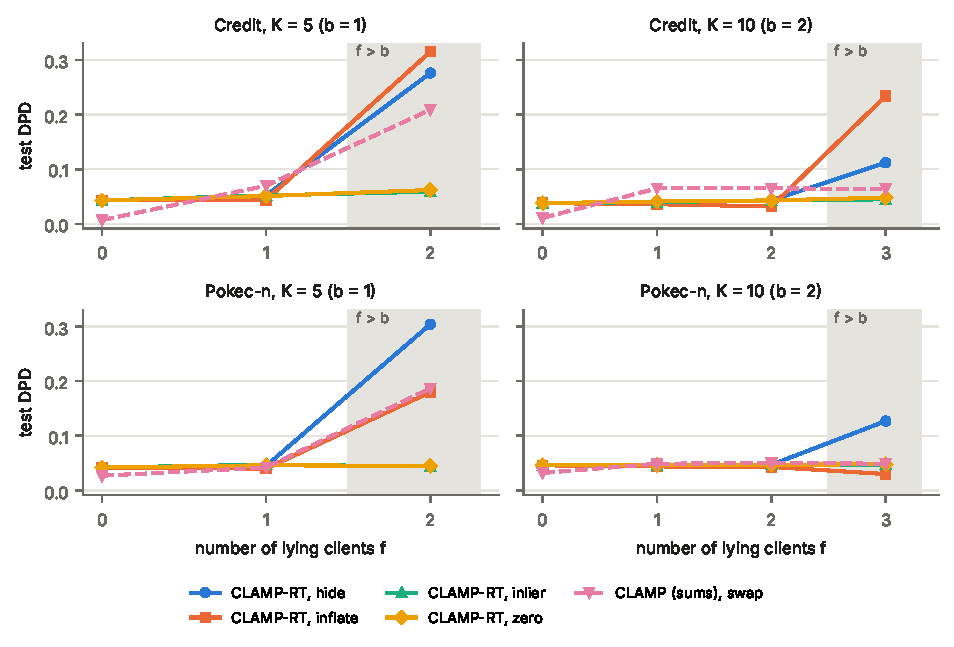
\includegraphics[width=\linewidth]{figures/fig_liars}
\caption{Test $\dpd$ against the number of lying clients $f$ (mean over 3 seeds). Shaded: $f>b$, beyond the breakdown point of the trimmed channel. Dashed: \clamp{} (sums channel, $P=1$) under the swap attack.}\label{fig:liars}
\end{figure}

\paragraph{Up to the breakdown point, liars have no measurable effect}
Table~\ref{tab:e4} and Figure~\ref{fig:liars} report the four gap attacks. For every dataset, $K$, attack and $f\le b$, the mean test gap stays within 0.009 of the honest run with the same seeds, which is less than its seed-to-seed standard deviation; the largest change is on Credit with $K=5$ and one hiding client (0.043 to 0.052). AUC changes by less than 0.01 (Table~S1). In all \nTthreeRounds{} attacked release rounds with $f\le b$ the pre-noise trimmed mean lay inside the interval of Theorem~\ref{thm:falsify}, as it must; this checks the implementation, not the theorem.

\paragraph{Beyond the breakdown point, the hiding and inflating attacks succeed}
With $f=b+1$ one false value survives the trimming. The \emph{hide} attack, which reports a gap of full size with the opposite sign, then flips the sign of the estimate, and the controller pushes the model the wrong way: the gap rises to 0.276--0.304 with $K=5$ and to 0.112--0.127 with $K=10$ on Credit and the Pokec graphs, above the unconstrained level. The \emph{inflate} attack forces over-correction; on Credit it raises the gap to 0.315 ($K=5$) and 0.234 ($K=10$) and costs 0.09--0.14 AUC, whereas on the Pokec graphs with $K=10$ it lowers the gap below the honest level (0.015 and 0.030) at a cost of about 0.01 AUC. The \emph{inlier} and \emph{zero} attacks, whose claims stay close to the honest values, have no clear effect even beyond the breakdown point (at most 0.062 against 0.043 on Credit). On Bail, where the budget does not bind, no attack has an effect.

\paragraph{Comparison with the sums channel}
Table~\ref{tab:oldnew} compares the two channels. With the sums channel a single liar out of ten raised the gap from \oldCreditKtenHon{} to \oldCreditKtenOne{} on Credit, from \oldPokeczKtenHon{} to \oldPokeczKtenOne{} on Pokec-z and from \oldPokecnKtenHon{} to \oldPokecnKtenOne{} on Pokec-n, i.e.\ to roughly the level of training without control, and additional liars did not change this. With the trimmed channel, one or two liars out of ten leave the gap at the honest level. The comparison has to be read with Table~\ref{tab:e1} in mind: because the honest level of \rt{} is itself higher, the attacked gap of \rt{} is lower than the attacked gap of \clamp{} only on Credit (0.041 against 0.065 for $f=1$, $K=10$); on the Pokec graphs the two are equal (0.046 against 0.045 and 0.049). What \rt{} gains is predictability: up to $b$ liars, its fairness under attack is its fairness without attack. With $K=5$ and two liars both channels fail.

\subsection{Update attacks and fairness poisoning}\label{sec:byz}

\begin{table}[tbp]
\centering
\scriptsize
\setlength{\tabcolsep}{3pt}
\caption{Fairness poisoning through updates ($K=10$): test DPD (AUC in parentheses), mean over 3 seeds. Baselines and CLAMP (sums channel, $P=1$) are from the earlier study; $^\dagger$ needs individual updates and cannot run under secure aggregation. CLAMP-RT uses $P=10$.}
\label{tab:e3}
\begin{adjustbox}{max width=\textwidth}
\begin{tabular}{lcccccccc}
\toprule
Dataset & $f$ & FedAvg & Median$^\dagger$ & TrMean$^\dagger$ & Krum$^\dagger$ & ClipMean & CLAMP & CLAMP-RT \\
\midrule
Pokec-z & 0 & 0.035 (0.75) & 0.033 (0.75) & 0.035 (0.74) & 0.033 (0.74) & 0.045 (0.76) & 0.028 (0.76) & 0.046 (0.77) \\
 & 1 & 0.062 (0.75) & 0.046 (0.74) & 0.047 (0.73) & 0.035 (0.74) & 0.065 (0.76) & 0.025 (0.76) & 0.059 (0.77) \\
 & 2 & 0.124 (0.71) & 0.108 (0.72) & 0.146 (0.70) & 0.034 (0.72) & 0.137 (0.75) & 0.037 (0.72) & 0.118 (0.75) \\
 & 3 & 0.137 (0.70) & 0.148 (0.72) & 0.186 (0.69) & 0.035 (0.73) & 0.172 (0.74) & 0.049 (0.71) & 0.151 (0.74) \\
 & 4 & 0.137 (0.69) & 0.111 (0.72) & 0.201 (0.71) & 0.086 (0.71) & 0.125 (0.73) & 0.047 (0.71) & 0.106 (0.73) \\
\midrule
Bail & 0 & 0.011 (0.76) & 0.007 (0.73) & 0.013 (0.75) & 0.003 (0.72) & 0.009 (0.75) & 0.011 (0.75) & 0.009 (0.74) \\
 & 1 & 0.008 (0.75) & 0.008 (0.72) & 0.014 (0.74) & 0.005 (0.72) & 0.011 (0.74) & 0.012 (0.74) & 0.010 (0.74) \\
 & 2 & 0.014 (0.72) & 0.009 (0.72) & 0.010 (0.73) & 0.009 (0.71) & 0.010 (0.72) & 0.011 (0.72) & 0.009 (0.72) \\
 & 3 & 0.018 (0.71) & 0.010 (0.72) & 0.012 (0.73) & 0.005 (0.71) & 0.016 (0.72) & 0.009 (0.72) & 0.015 (0.71) \\
 & 4 & 0.021 (0.70) & 0.013 (0.71) & 0.014 (0.72) & 0.009 (0.71) & 0.023 (0.71) & 0.014 (0.72) & 0.023 (0.71) \\
\bottomrule
\end{tabular}
\end{adjustbox}
\end{table}


The trimmed channel does not change the update channel, and the results confirm it. Under the four update attacks that target utility, \rt{} behaves like the clipped mean of the earlier study (Table~S2): scaling has no effect because scaled updates are clipped; sign flipping lowers AUC gradually from 0.743 to 0.661 on Bail and from 0.768 to 0.710 on Pokec-z as $f$ grows from 0 to 4; ALIE and IPM cost at most 0.033 AUC.

Fairness poisoning is different (Table~\ref{tab:e3}). On Pokec-z it raises the gap of \rt{} to 0.118, 0.151 and 0.106 for $f=2,3,4$, close to ClipMean (0.137, 0.172, 0.125) and FedAvg (0.124--0.137). \clamp{} with per-round releases held the same attack at 0.037--0.049. In this respect \rt{} is a regression. The poisoning clients report their true gaps, so the gap channel does see the growing gap, but the multiplier of \rt{} reached at most 0.39 at the end of these runs, whereas that of \clamp{} reached 0.56--4.04 in eight of its nine runs with $f\ge2$. We attribute the difference mainly to the release period ($P=10$ gives the controller ten updates instead of a hundred), but we did not run \rt{} with $P=1$ under this attack, so this explanation is untested. Among the rules that need individual updates, only Krum held the gap (0.034--0.035 up to $f=3$). On Bail the attack raises the gap of every method by at most 0.014.

\subsection{Cost of the secure computation}\label{sec:mpc}

\begin{table}[tbp]
\centering
\footnotesize
\setlength{\tabcolsep}{4pt}
\caption{Measured cost of one release round of the server-side protocol in semi-honest two-party computation (CrypTen, two processes on one machine, local network; median of 3 repetitions). Bytes are those sent by one server as reported by CrypTen; rounds are communication rounds. Update channel: norm checks and masked sum of $K$ updates of dimension $d$. Gap channel: range checks, sort, trimmed mean and noise addition. Err: largest absolute fixed-point error of the trimmed mean (noise switched off). Client-to-server input sharing is not included.}
\label{tab:mpc}
\begin{adjustbox}{max width=\textwidth}
\begin{tabular}{rrr rrr rrrr}
\toprule
 & & & \multicolumn{3}{c}{Update channel} & \multicolumn{4}{c}{Gap channel} \\
$K$ & $b$ & $d$ & MB & rounds & s & KB & rounds & s & Err \\
\midrule
5 & 1 & $10^{4}$ & 2.56 & 12 & 0.79 & 9.3 & 64 & 0.33 & 5.9$\times10^{-6}$ \\
5 & 1 & $10^{5}$ & 25.60 & 12 & 1.44 & 9.3 & 64 & 0.30 & 1.0$\times10^{-5}$ \\
5 & 1 & $10^{6}$ & 256.00 & 12 & 3.12 & 9.3 & 64 & 0.33 & 1.5$\times10^{-5}$ \\
10 & 2 & $10^{4}$ & 4.96 & 12 & 0.88 & 30.2 & 109 & 0.54 & 1.0$\times10^{-5}$ \\
10 & 2 & $10^{5}$ & 49.60 & 12 & 1.33 & 30.2 & 109 & 0.51 & 1.1$\times10^{-5}$ \\
10 & 2 & $10^{6}$ & 496.00 & 12 & 4.51 & 30.2 & 109 & 0.42 & 6.4$\times10^{-6}$ \\
20 & 4 & $10^{4}$ & 9.77 & 12 & 0.73 & 106.7 & 199 & 0.92 & 9.7$\times10^{-6}$ \\
20 & 4 & $10^{5}$ & 97.61 & 12 & 1.47 & 106.7 & 199 & 1.12 & 1.2$\times10^{-5}$ \\
20 & 4 & $10^{6}$ & 976.01 & 12 & 9.55 & 106.7 & 199 & 0.95 & 1.5$\times10^{-5}$ \\
\bottomrule
\end{tabular}
\end{adjustbox}
\end{table}


We implemented the server step (validity checks, masked update sum, sort, trimming and noise) in CrypTen~\citep{knott2021crypten}: semi-honest two-party computation over $\mathbb{Z}_{2^{64}}$ with 16 fractional bits, Beaver triples from a trusted dealer, two processes on one machine, and an odd-even transposition sorting network ($K$ passes). Table~\ref{tab:mpc} reports one release round.

The gap channel does not depend on the model size. It takes 64, 109 and 199 communication rounds and 9.3, 30.2 and 106.7\,KB for $K=5$, 10 and 20 clients, and 0.30--1.12\,s on the local machine. The update channel takes 12 rounds for any size, and its traffic grows linearly with $K\cdot d$: 4.96\,MB and 0.88\,s for $K=10$, $d=10^4$, and 496\,MB and 4.5\,s for $d=10^6$. In the gap channel the round count dominates over a wide-area network; at 50\,ms round-trip time, 199 rounds would add about 10\,s per release, a figure we computed and did not measure. The largest fixed-point error of the trimmed mean was $1.5\times10^{-5}$, three orders of magnitude below $\sigma_d$ on every dataset.

The measurement has clear limits. It is semi-honest, so a server that deviates from the protocol is not covered; ELSA-style malicious security~\citep{rathee2023elsa} would cost more. The trusted dealer and the clients' input sharing are not included. The noise was switched off in the error measurement, and the noise of the protocol is a continuous Gaussian sampled in floating point and then shared, not a discrete mechanism over the ring. A sorting network with lower depth than odd-even transposition would reduce the round count for larger $K$; we did not implement one. Finally, the training experiments did not run inside CrypTen; they execute the same arithmetic in plaintext.

\subsection{Privacy}\label{sec:privacy}

\begin{table}[tbp]
\centering
\footnotesize
\caption{Balanced accuracy of the optimal test that distinguishes two attribute-neighbouring datasets from the released gap (closed form, worst case $|\Delta|=\Delta_{\mathrm{TM}}$; $R=10$ releases, $\delta=10^{-5}$). $z=\sigma_d/\Delta_{\mathrm{TM}}$ from the RDP calibration. Both servers honest: one release with variance $2\sigma_d^2$. One server colluding: it removes its own noise. All releases: the colluding server combines all $R$ releases of a target whose contribution is unchanged. Bound: $(e^{\varepsilon}+\delta)/(1+e^{\varepsilon})$.}
\label{tab:attack}
\begin{adjustbox}{max width=\textwidth}
\begin{tabular}{cccccc}
\toprule
$\varepsilon$ & $z$ & Both honest, one release & One server, one release & One server, all $R$ & Bound \\
\midrule
1 & 12.79 & 0.511 & 0.516 & 0.549 & 0.7311 \\
2 & 6.80 & 0.521 & 0.529 & 0.592 & 0.8808 \\
4 & 3.66 & 0.538 & 0.554 & 0.667 & 0.9820 \\
8 & 2.02 & 0.570 & 0.598 & 0.783 & 0.9997 \\
\bottomrule
\end{tabular}
\end{adjustbox}
\end{table}

\begin{table}[tbp]
\centering
\scriptsize
\setlength{\tabcolsep}{3pt}
\caption{Privacy budget $\varepsilon$ of the gap channel and release period $P$ ($K=5$, 3 seeds): test DPD, mean$\pm$sd. All other experiments use $\varepsilon=8$ and $P=10$.}
\label{tab:e5}
\begin{adjustbox}{max width=\textwidth}
\begin{tabular}{cccccccccc}
\toprule
 & \multicolumn{3}{c}{Credit} & \multicolumn{3}{c}{Pokec-z} & \multicolumn{3}{c}{Pokec-n} \\
$\varepsilon$ & $P=1$ & $P=5$ & $P=10$ & $P=1$ & $P=5$ & $P=10$ & $P=1$ & $P=5$ & $P=10$ \\
\midrule
1 & 0.057$\pm$0.022 & 0.057$\pm$0.007 & 0.063$\pm$0.005 & 0.051$\pm$0.027 & 0.056$\pm$0.012 & 0.046$\pm$0.007 & 0.055$\pm$0.039 & 0.055$\pm$0.026 & 0.048$\pm$0.009 \\
2 & 0.056$\pm$0.023 & 0.060$\pm$0.004 & 0.066$\pm$0.006 & 0.046$\pm$0.023 & 0.048$\pm$0.005 & 0.045$\pm$0.006 & 0.049$\pm$0.024 & 0.051$\pm$0.017 & 0.044$\pm$0.007 \\
4 & 0.061$\pm$0.019 & 0.063$\pm$0.003 & 0.049$\pm$0.027 & 0.030$\pm$0.004 & 0.045$\pm$0.002 & 0.039$\pm$0.006 & 0.032$\pm$0.005 & 0.043$\pm$0.004 & 0.043$\pm$0.012 \\
8 & 0.090$\pm$0.056 & 0.062$\pm$0.003 & 0.044$\pm$0.019 & 0.028$\pm$0.002 & 0.038$\pm$0.006 & 0.041$\pm$0.003 & 0.029$\pm$0.003 & 0.041$\pm$0.011 & 0.043$\pm$0.014 \\
\bottomrule
\end{tabular}
\end{adjustbox}
\end{table}


\begin{figure}[tbp]
\centering
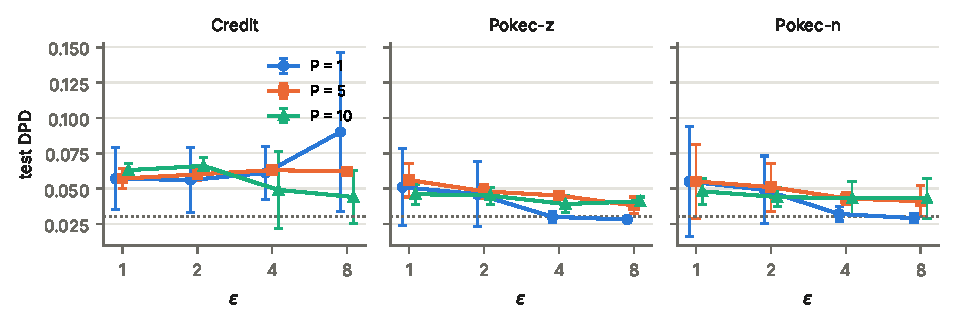
\includegraphics[width=\linewidth]{figures/fig_privacy}
\caption{Test $\dpd$ of \rt{} against the privacy budget of the gap channel for three release periods (mean $\pm$ sd over 3 seeds; dotted: budget $\tau=0.03$).}\label{fig:privacy}
\end{figure}

\paragraph{What the released gap reveals}
For a single release, the best test between two neighbouring datasets observes $\gt$ with mean $\TM$ or $\TM+\Delta$, $|\Delta|\le\DTM$, and noise $\mathcal{N}(0,2\sigma_d^2)$; its balanced accuracy is $\Phi(\Delta/(2\sqrt2\sigma_d))\le\Phi(1/(2\sqrt2 z))$, independent of the dataset because $\sigma_d=z\DTM$. Table~\ref{tab:attack} evaluates it. At $\varepsilon=8$ it is \accBothEight{} with both servers honest, \accOneEight{} if one server colludes and removes its own noise, and \accAllEight{} if the colluding server also combines all ten releases of a node whose contribution does not change, the worst case the accounting covers. The $(\varepsilon,\delta)$ bound, $(e^\varepsilon+\delta)/(1+e^\varepsilon)=\boundEight$, is uninformative at this level; the closed form is the more useful description. These values are for the worst case $|\Delta|=\DTM$; a node in a group much larger than $n_{0,k}$ changes the trimmed mean by less.

\paragraph{Privacy budget and release period}
Table~\ref{tab:e5} and Figure~\ref{fig:privacy} vary $\varepsilon$ and $P$. On Pokec-z and Pokec-n, per-round releases work best once $\varepsilon\ge4$ (0.028--0.032), matching \clamp{}, while $P=10$ stays at 0.039--0.043; at $\varepsilon\le2$ all periods give 0.044--0.056. On Credit no setting reaches the budget: the gap is 0.044--0.090, with the largest values and spread at $P=1$, $\varepsilon=8$ (0.090 $\pm$ 0.056), and at $\varepsilon\le4$ the results are noisy at every period. AUC is \eFiveAucMin--\eFiveAucMax{} throughout (Table~S4). Our uniform choice $P=10$ is therefore not the best choice on the Pokec graphs. We nevertheless report all other experiments with $P=10$, because no single period was better on all three graphs.

\paragraph{What the model reveals}
Theorem~\ref{thm:dp} does not cover the trained model. The earlier study probed the final models of FedAvg, ClipMean and \clamp{} (last iterate) with a logistic-regression attribute probe on hidden representations: on German the probe reached AUC 0.86--0.87 for all three, against 0.85 for the raw features and 0.91 for an untrained GAT, and on Bail 0.54 against 0.61 for the raw features. We did not repeat the probe for \rt{}. Its model is trained by the same loop with a different multiplier, and we expect, but have not verified, similar values. Demographic-parity control does not remove the attribute from the representation, and neither protocol claims that it does.

\subsection{Ablations}\label{sec:ablation}

\begin{table}[tbp]
\centering
\footnotesize
\setlength{\tabcolsep}{3pt}
\caption{Ablations of the trimmed channel ($K=5$, $\varepsilon=8$, $P=10$, 3 seeds, honest). These runs use the variant without bias correction. $\sigma_d$ is the per-server noise standard deviation (mean$\pm$sd over seeds).}
\label{tab:e6}
\begin{adjustbox}{max width=\textwidth}
\begin{tabular}{l ccc ccc}
\toprule
 & \multicolumn{3}{c}{Credit} & \multicolumn{3}{c}{Pokec-z} \\
Variant & AUC & DPD & $\sigma_d$ & AUC & DPD & $\sigma_d$ \\
\midrule
Default ($b=1$, $c=0.05$) & 0.755$\pm$0.012 & 0.026$\pm$0.017 & 0.063$\pm$0.014 & 0.754$\pm$0.032 & 0.041$\pm$0.001 & 0.028$\pm$0.002 \\
Last iterate (no output rule) & 0.750$\pm$0.014 & 0.031$\pm$0.023 & 0.063$\pm$0.014 & 0.748$\pm$0.027 & 0.036$\pm$0.001 & 0.028$\pm$0.002 \\
$b=0$ (plain mean, no robustness) & 0.762$\pm$0.007 & 0.027$\pm$0.008 & 0.038$\pm$0.008 & 0.752$\pm$0.027 & 0.039$\pm$0.002 & 0.017$\pm$0.001 \\
$b=2$ (median of $K=5$) & 0.683$\pm$0.041 & 0.168$\pm$0.048 & 0.188$\pm$0.042 & 0.752$\pm$0.038 & 0.039$\pm$0.021 & 0.084$\pm$0.005 \\
$c=0.2$ & 0.657$\pm$0.004 & 0.236$\pm$0.008 & 0.016$\pm$0.004 & 0.753$\pm$0.026 & 0.033$\pm$0.004 & 0.007$\pm$0.000 \\
\bottomrule
\end{tabular}
\end{adjustbox}
\end{table}


Table~\ref{tab:e6} varies the trimming level, the floor fraction and the output rule on Credit and Pokec-z (variant without bias correction, three seeds). Trimming costs little in honest runs: the plain mean ($b=0$) has a smaller $\sigma_d$ (0.038 against 0.063 on Credit) and a gap within seed noise of the default (0.027 against 0.026). Two settings are clearly bad. With $b=2$ at $K=5$ the statistic is the median, its sensitivity triples ($\sigma_d=0.188$ on Credit), and the Credit gap rises to 0.168 with AUC 0.683. With $c=0.2$ the noise is smaller ($\sigma_d=0.016$), but the Credit gap is 0.236 with AUC 0.657. The likely reason is the floor: the protected group is 9\% of Credit's nodes, so with $c=0.2$ it is smaller than $n_{0,k}$ on most clients, its rate is shrunk toward zero, and the estimated gap is biased in one direction; on Pokec-z, whose groups are larger than the floor, $c=0.2$ works (0.033). The floor fraction must therefore stay below the smallest group share, which is a constraint the federation has to set from public knowledge. Returning the last iterate instead of the stored model changes the gap by less than the seed noise in these runs (0.031 against 0.026 on Credit, 0.036 against 0.041 on Pokec-z).
